\documentclass[12pt]{article}
\usepackage[T1, T2A]{fontenc}
\usepackage[utf8]{inputenc}
\usepackage[russian]{babel}
\usepackage{hyperref}
\usepackage{graphicx}
\graphicspath{ {../Images/} }

\author{Григорий Матюхин}
\date{\today}
\title{Лабораторная работа \textnumero15.\\Управление логическими томами}

\begin{document}
\maketitle
\newpage
\tableofcontents
\newpage
\section{Цель работы}
Получить навыки управления логическими томами.

\section{Последовательность выполнения работы}
\subsection{Создание физического тома}
\begin{enumerate}
	\item В терминале с полномочиями администратора с помощью \texttt{fdisk} создайте основной раздел с типом LVM:
	      \\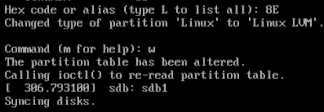
\includegraphics{4.png}
	\item Обновите таблицу разделов:
	\item Теперь, когда раздел был создан, вы должны укажите его как физический том LVM:
	\item Убедитесь, что физический том создан успешно:
	      \\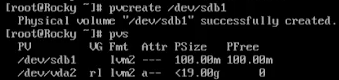
\includegraphics{5.png}
\end{enumerate}

\subsection{Создание группы томов и логических томов}
\begin{enumerate}
	\item В терминале с полномочиями администратора проверьте доступность физических
	      томов в вашей системе:
	\item Создайте группу томов с присвоенным ей физическим томом:
	\item Убедитесь, что группа томов была создана успешно:
	      \\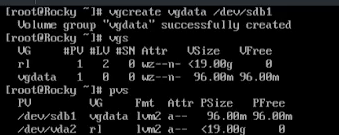
\includegraphics{6.png}
	\item Создайте логический том LVM с именем \texttt{lvdata}, который будет использовать
	      50\% доступного дискового пространства в группе томов \texttt{vgdata}:
	\item Проверьте успешность добавления тома:
	      \\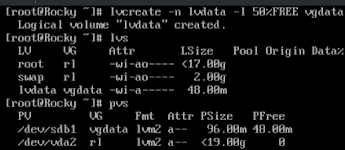
\includegraphics{7.png}
	\item Создайте файловую систему поверх тома:
	\item Создайте директорию, на которую можно смонтировать том:
	\item Добавьте следующую строку в \texttt{/etc/fstab} \texttt{/dev/vgdata/lvdata /mnt/data ext4 defaults 1 2}:
	\item Проверьте, монтируется ли файловая система:
	      \\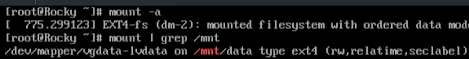
\includegraphics{9.png}
\end{enumerate}

\subsection{Изменение размера логических томов}
\begin{enumerate}
	\item В терминале с полномочиями администратора введите \texttt{pvs} и \texttt{vgs}, чтобы отобразить
	      текущую конфигурацию физических томов и группы томов.
	\item С помощью \texttt{fdisk} добавьте раздел \texttt{/dev/sdb2} размером 100 М. Задайте тип раздела \texttt{8e}:
	      \\
\includegraphics{10.png}
	\item Создайте физический том:
	\item Расширьте \texttt{vgdata}:
	\item Проверьте, что размер доступной группы томов увеличен:
	      \\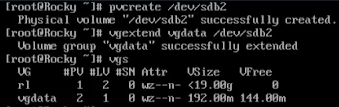
\includegraphics{11.png}
	\item Увеличьте \texttt{lvdata} на 50\% оставшегося доступного дискового пространства в группе томов:
	\item Убедитесь, что добавленное дисковое пространство стало доступным:
	      \\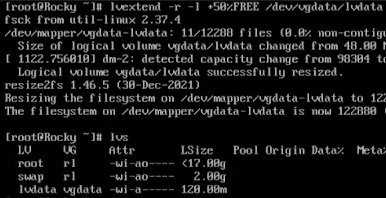
\includegraphics{12.png}
	\item Уменьшите размер \texttt{lvdata} на 50 МБ:
	\item Убедитесь в успешном изменении дискового пространства:
	      \\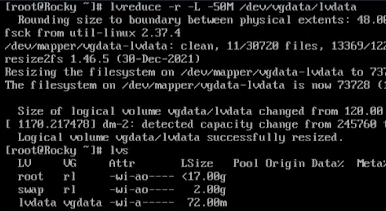
\includegraphics{13.png}
\end{enumerate}


\subsection{Самостоятельная работа}
\begin{enumerate}
	\item Создайте логический том \texttt{lvgroup} размером 200 МБ. Отформатируйте его в
	      файловой системе XFS и cмонтируйте его постоянно на \texttt{/mnt/groups}. Перезагрузите
	      виртуальную машину, чтобы убедиться, что устройство подключается.
	      \\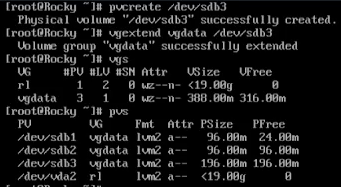
\includegraphics{14.png}
	      \\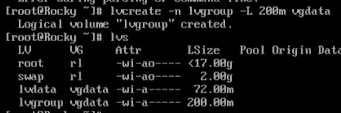
\includegraphics{15.png}
	      \\
\includegraphics{16.png}
	      \\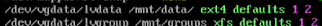
\includegraphics{17.png}
	      \\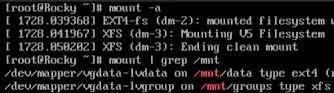
\includegraphics{18.png}
	\item После перезагрузки добавьте ещё 150 МБ к тому \texttt{lvgroup}. Убедитесь, что размер
	      файловой системы также изменится при изменении размера тома.
	      \\
\includegraphics{19.png}
	\item Убедитесь, что расширение тома выполнено успешно.
	      \\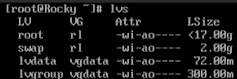
\includegraphics{20.png}
\end{enumerate}

\section{Контрольные вопросы}
\begin{enumerate}
	\item Какой тип раздела используется в разделе GUID для работы с LVM? \\
	      Linux LVM
	\item Какой командой можно создать группу томов с именем \texttt{vggroup}, которая содержит
	      физическое устройство \texttt{/dev/sdb3} и использует физический экстент 4 MiB? \\
	      \texttt{vgcreate vggroup /dev/sdb3 -s 4m}
	\item Какая команда показывает краткую сводку физических томов в вашей системе,
	      а также группу томов, к которой они принадлежат? \\
	      \texttt{vps}
	\item Что вам нужно сделать, чтобы добавить весь жёсткий диск \texttt{/dev/sdd} в группу
	      томов \texttt{groups}? \\
	      \texttt{pvcreate /dev/sdd} \\
	      \texttt{vgextend groups /dev/sdd}
	\item Какая команда позволяет вам создать логический том \texttt{lvvol1} с размером 6 MiB? \\
	      \texttt{lvcreate lvvol1 -L 6m <group-name>}
	\item Какая команда позволяет вам добавить 100 МБ в логический том \texttt{lvvol1}, если
	      предположить, что дисковое пространство доступно в группе томов?
	      \texttt{lvextend -r -L +50m <path-to-lvvol1>}
	\item Каков первый шаг, чтобы добавить ещё 200 МБ дискового пространства в
	      логический том, если требуемое дисковое пространство недоступно в группе томов? \\
	      Расширить группу томов.
	\item Какую опцию нужно использовать с командой \texttt{lvextend}, чтобы также изменить
	      размер файловой системы? \\
	      \texttt{--fs resize}
	\item Как посмотреть, какие логические тома доступны? \\
	      \texttt{lvs}
	\item Какую команду нужно использовать для проверки целостности файловой системы
	      на \texttt{/dev/vgdata/lvdata}? \\
	      \texttt{df -h}
\end{enumerate}

\section{Вывод}
В ходе выполнения данной работы я получил навыки управления логическими томами.

\end{document}
